%%%%%%%%%%%%%%%%%%%%%%%%%%%%%%%%%%%%%%%%%%%%%%%%%%%%%%%%%%%%%%%%%%%%%%%%%%%%%%%
%%%%%%%%%%%%%%%%%%%%%%%%%%%%%%%%%%%%%%%%%%%%%%%%%%%%%%%%%%%%%%%%%%%%%%%%%%%%%%%
%%%%  CHAPTER 8
%%%%%%%%%%%%%%%%%%%%%%%%%%%%%%%%%%%%%%%%%%%%%%%%%%%%%%%%%%%%%%%%%%%%%%%%%%%%%%%
%%%%%%%%%%%%%%%%%%%%%%%%%%%%%%%%%%%%%%%%%%%%%%%%%%%%%%%%%%%%%%%%%%%%%%%%%%%%%%%
\chapter{Diagnostic tools III:  Double occupancy}

As we saw in Chapter~\ref{chap:hubbardmodel}, an important thermodynamic
quantity in the Hubbard model is the double occupancy.  Detailed studies of
this quantity have been used to demonstrate the achievement of a Mott
insulating regime~\cite{Jordens2008,Schneider2008}, to extract the
compressibility of fermions in a lattice ~\cite{Scarola2009},  and to measure
temperature and entropy via comparison with theoretical
calculations~\cite{Jordens2010b}.  Measurements of the double occupancy in an
optical lattice have been achieved mainly by two methods: using Feshbach
resonances to spectroscopically differentiate the singly and doubly occupied
sites~\cite{RevModPhys.82.1225}, or using one-color photoassociation, which
selectively expels atoms in doubly occupied sites from the
trap~\cite{PhysRevLett.93.073002} (and then measuring the remaining atom
number).

Measurements of the double occupancy using one-color photoassociation to an
excited molecular state were first performed on bosonic
atoms~\cite{PhysRevLett.93.073002,PhysRevLett.96.050402}, but have also been
realized for fermionic $^{173}$Yb~\cite{Taie2012}. This technique requires a
dedicated laser tuned to the excited molecular state (which can be several
hundred GHz away from the excited state of free atoms).  In our experiment we
did not have the required frequency readily available, so we implemented
double occupancy measurements using the Feshbach resonance technique. 

The presence of more than one Feshbach resonance for a pair of hyperfine
states, or Feshbach resonances at different magnetic fields for spin mixtures
in different hyperfine states,  can be exploited in a variety of ways to
measure double occupancies in an optical lattice.    The possibilities depend
on the scattering properties of the atom used.   Previous experiments with
$^{40}$K atoms~\cite{Jordens2010,Schneider2010}  have used Feshbach resonances
to  measure the double occupancy.  In $^{40}$K, repulsive interactions are
realized with a spin mixture of atoms in the $m_{F}=-5/2$ and $m_{F}=-9/2$
hyperfine states, with total angular momentum $F=9/2$.   A Feshbach resonance
between the $m_{F}=-9/2$ and $m_{F}=-7/2$ spin states can be used to shift the
energy required to flip the spin of an $m_{F}=-5/2$ atom.    If such an atom is
in a singly occupied state it can be flipped to $m_{F}=-7/2$ by driving a
$\pi$-pulse at a frequency $f_{\mathrm{single}}$. If it is in a doubly occupied
site,  flipping the spin to $m_{F}=-7/2$ will create a bound state, so the RF
spin flip resonance is shifted by the binding energy: $f_{\mathrm{double}} =
f_{\mathrm{single}} + E_{\mathrm{binding}}/h$.  In such a way, one can
selectively change the spin of $m_{F}=-5/2$ atoms only if they are in a doubly
occupied site~\cite{PhysRevLett.96.030401}.    After doing this, the atoms are
released in TOF, applying a strong magnetic field gradient to effect a
Stern-Gerlach separation of the populations in the different spin states.
Once separated the different populations can be imaged and counted, giving the
double occupancy in the lattice. 

The same procedure will not work in \li for two reasons.  The first one has to
do with the scattering properties of \li, which we will review in a moment.
The second one is simply because lithium is a light atom, and it expands
quickly in TOF.  It is then challenging to resolve the different spin states in
a Stern-Gerlach separation measurement.




\section{\li\ Feshbach resonances}

Figure~\ref{fig:ajochim} shows the scattering length between \li\ atoms in
states $|1\rangle$ and $|2\rangle$ (see the energy level diagram in
Fig.~\ref{fig:zeemanlevels} for reference) as a function of magnetic field.
Most of our experiments take place in the range between $550\,$G and $650\,$G,
to the right of the narrow Feshbach resonance (little bump in the plot) present
at 543.3~G~\cite{Strecker2003,Hazlett2012}.   Within this range, the scattering
length is $<800\,a_{0}$, avoiding larger values where  significant collisional
losses are observed.
\begin{figure}
\centering
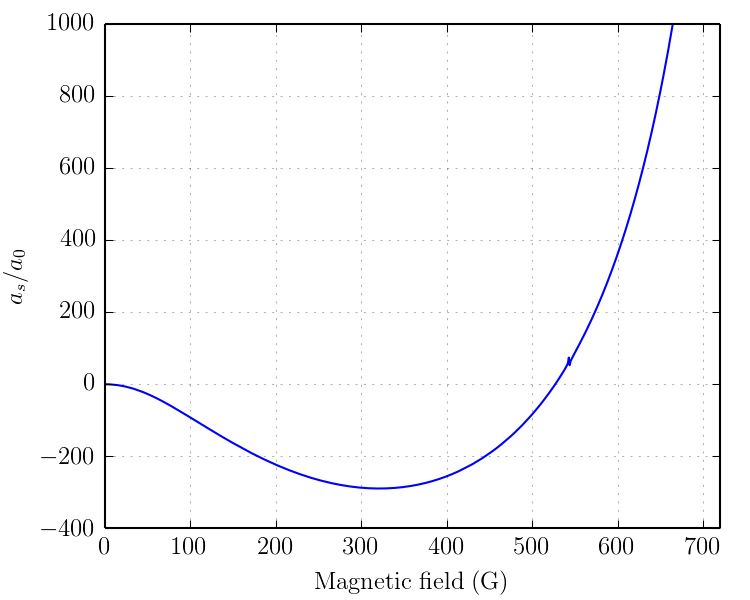
\includegraphics[width=0.55\textwidth]{../figures/double_occ/ajochim_plot.png}
\caption[\li\ scattering length vs. magnetic field]{Scattering length between
\li\ atoms in states $|1\rangle$ and $|2\rangle$ vs. magnetic field in Gauss.
A broad Feshbach resonance is centered at 832~G and a narrow Feshbach resonance
is centered at 543.3~G~\cite{Strecker2003,Hazlett2012}.  The data for this plot
was obtained from Ref.~\cite{Zurn2013}.}
\label{fig:ajochim}
\end{figure}


To give rise to a virtual molecular bound state that can be used to selectively
flip the spins of atoms in singly and doubly occupied sites, one needs to
approach a Feshbach resonance between a different pair of hyperfine states
($|1\rangle$, $|3\rangle$ or $|2\rangle$, $|3\rangle$ in our case)  from the
attractive to the repulsive side.   The broad resonances between $|1\rangle$,
$|3\rangle$, and $|2\rangle$, $|3\rangle$ occur at 690~G and 811~G,
respectively, so within our operating field range we cannot cross any of these
resonances to exploit the binding energy of the virtual molecular state.
Nevertheless, as can be seen in Fig.~\ref{fig:ajochim}, we have at our disposal
the narrow Feshbach resonance between states $|1\rangle$ and $|2\rangle$, which
occurs at 543.3~G.  

In a narrow resonance, the molecular state that exists on the repulsive side of
the resonance becomes deeply bound for fields even a few Gauss away from the
resonance~\cite{Hazlett2012}.   In this case, the narrowness of the resonance
places a significant constraint on the stability of the magnetic field if one
is to exploit RF transitions in close proximity to the resonance.  However, the
binding energy of the molecular state away from the resonance is so large, that
atoms and molecules can be resolved spectroscopically with the \red\  optical
transition.  In addition, since the resonance is between states $|1\rangle$ and
$|2\rangle$ (the states we use in the experiment),  the molecular state is not
virtual.  If the field is ramped slowly across the resonance in the direction
of decreasing field, then atoms in doubly occupied sites will be associated to
form molecules with a probability very close to 1 due to the strong confinement
of a lattice site~\cite{Thalhammer2006}.  


\section{Measurement procedure} 

The sequence to measure the double occupancy using molecular association across
the Feshbach resonance proceeds as indicated in Fig.~\ref{fig:measure-doub}.
Below we list all the steps that are shown in the figure: 
\begin{itemize}
\item  The experiment starts out (in this example) at a field of 595~G
($a_{s}=326\,a_{0}$) and a lattice depth of 7\,$E_{r}$.  At $t=0$~ms, the
lattice depth is suddenly (in 1~ms) increased to 50\,$E_{r}$ (this lattice
depth ramp is not shown in the figure).  One could take an image at this time
(labeled as $\boxed{1}$ in the figure) to measure the total atom
number\footnote{Equivalently, the total atom number can also be measured before
locking the lattice.}  

\item During the lock ramp to 50\,$E_{r}$ each site is projected into a number
state, so singly and doubly occupied sites are well defined.  Additionally, in
the locked lattice the atoms are prevented from continuing to tunnel during the
duration of the double occupancy measurement.  The minimum duration of the
measurement determines the lattice depth requirements.  A few values of the
tunneling rate as a function of lattice depth are given in the table below.  We
will refer back to these in a moment, after explaining the entire measurement
procedure.
 
\vspace{0.5em}
\begin{centering}
 \begin{tabular}{c|cc}
      $V_{0}$ & $t$ (Hz)  & $1/t$ (ms) \\ 
      \hline
    7\,$E_{r}$  & 1153  & 0.867 \\  
    20\,$E_{r}$  & 73  & 13.7 \\ 
    50\,$E_{r}$  & 0.7  & 1412  \\
\end{tabular}
\end{centering}
\vspace{1em} 

\item  After locking the lattice, the scattering length is quickly ramped down
to  80~$a_{0}$ (547~G) in 8~ms.   The narrow resonance is then crossed using a
slow ramp that goes from 80 to 61 $a_{0}$ in 24~ms.  A slow ramp is required to
achieve nearly 100\% conversion efficiency of atoms in doubly occupied sites to
Feshbach molecules.  Notice that  ramps are linear in scattering length (we use
a calibration for the scattering length that ignores the narrow resonance) and
so the ramps are not exactly straight lines when showed in units of the
magnetic field, as in Fig.~\ref{fig:measure-doub}.  

\item After the field crosses the resonance, a 1~ms ramp takes the scattering
length down to 48\,$a_{0}$,  a field of $\approx 537.9$~G,  where the molecules
are dark.   At this point, labeled as $\boxed{2}$ in the figure, one could take
an image of atoms in singly occupied sites.  


\item In the short time that is spent below the resonance (time between points
$\boxed{2}$ and $\boxed{3}$) we proceed to blow away with resonant light any
atoms in singly occupied sites.  Two frequencies of light are needed in the
pulse, targeting atoms in spin states $|1\rangle$ and $|2\rangle$. 

\item After getting rid of atoms in singly occupied sites, the ramp across the
narrow resonance is reversed.  At a scattering length of 70\,$a_{0}$ ($\approx
545.1$~G), where the Feshbach molecules are dissociated, we can go ahead and
take a picture of atoms that were initially in doubly occupied sites.  That
point is labeled as $\boxed{4}$ in Fig.~\ref{fig:measure-doub}. 
\end{itemize}  
\begin{figure}
\centering
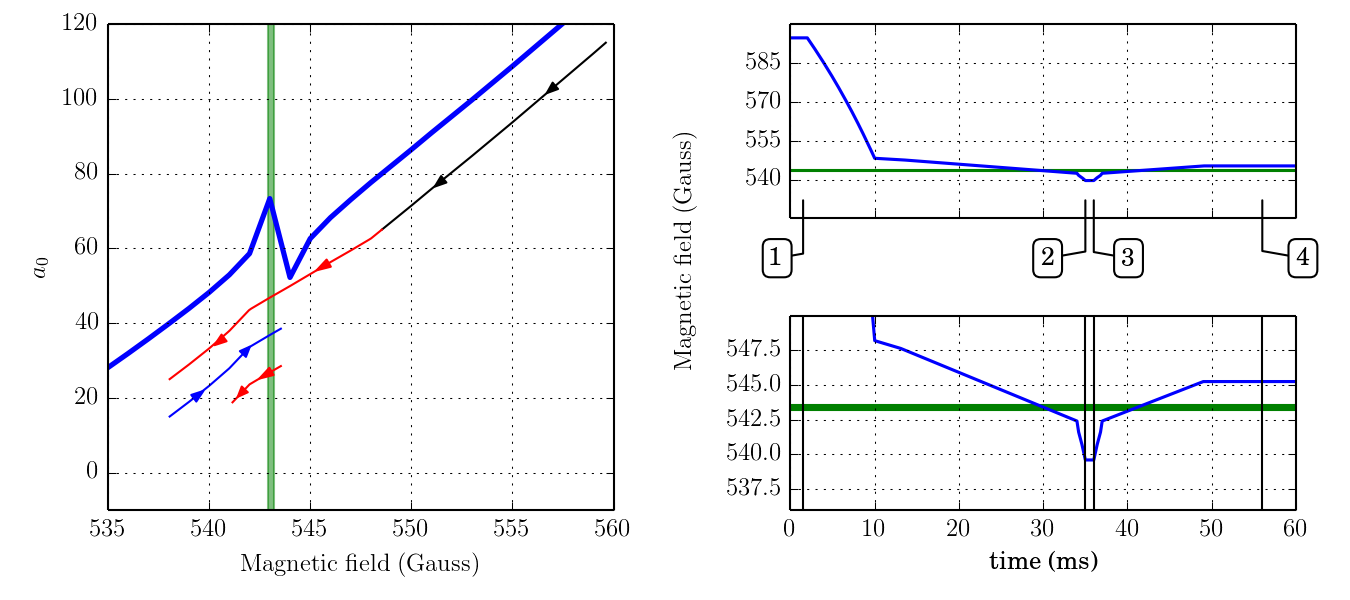
\includegraphics[width=\textwidth]{../figures/double_occ/narrowfr_sweeps2.png}
\caption[Double occupancy measurement]{Experimental sequence for measuring
double occupancy in an optical lattice.  The steps are explained in the text.
The direction of the magnetic field sweeps is shown by the colored lines with
arrows on the left plot. The change in color represents a different slope in
the field ramps.  } 
\label{fig:measure-doub}
\end{figure}

As one can see from the explanations above, several experiments are possible
depending on the time along these field ramps where one decides to image the
atoms.  For a direct image of the double occupancies, taken at point
$\boxed{4}$, at least $50$~ms are required for the field ramps involved in the
measurement. A locked lattice depth $V_{0}=43\,E_{r}$ is required to set a
limit of less that one tenth of a tunneling event during that time.

\section{Measurements in a compensated lattice} 

In Fig.~\ref{fig:docc-5.5Er} we show an example of the different measurements
explained above.  The sample is in the compensated lattice,   with lattice
depth set at $5.5\,E_{r}$ and the compensation set at $3\,E_{r}$.  The atom
number is $\sim\,$300,000 atoms.   
\begin{figure}
\centering
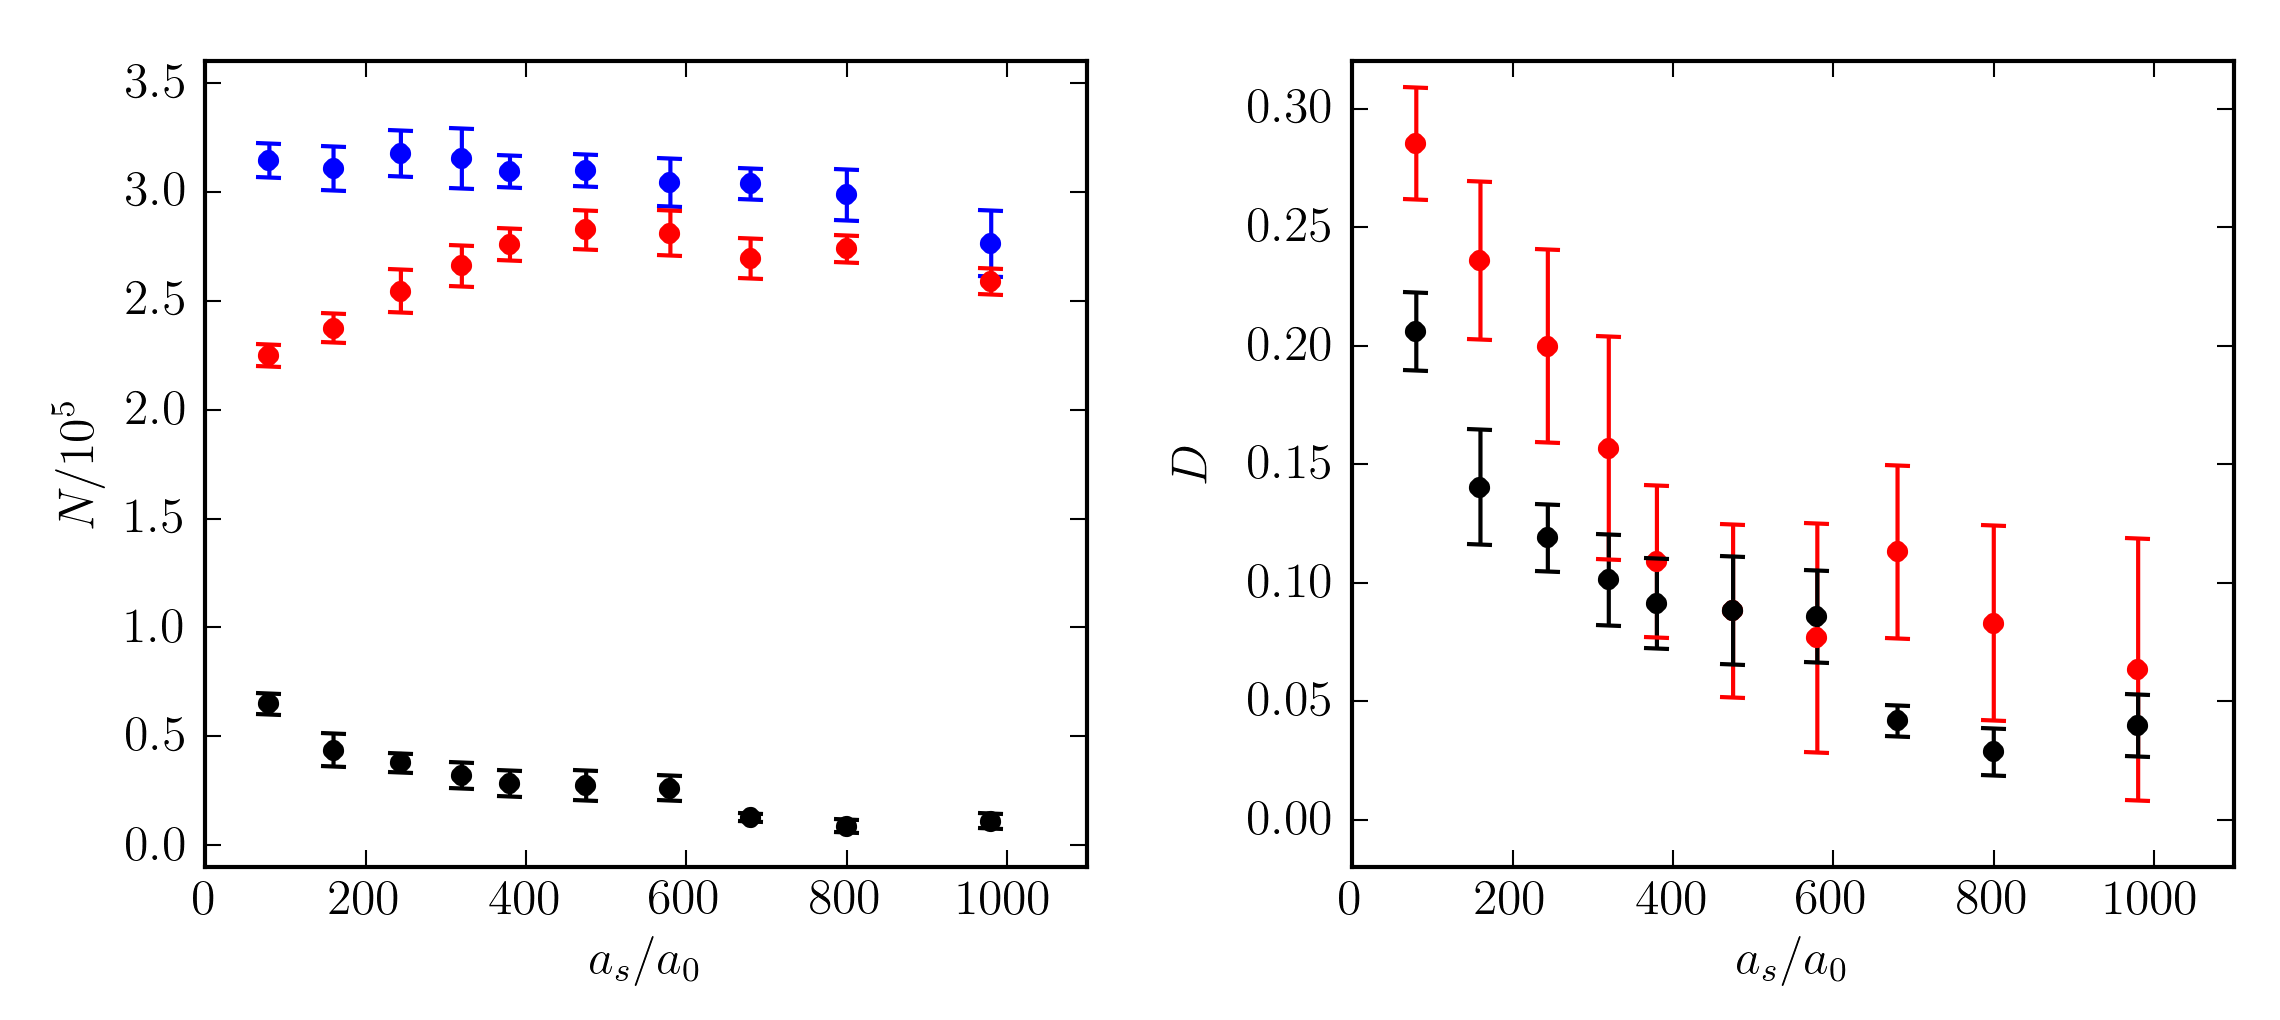
\includegraphics[width=\textwidth]{../figures/double_occ/insitu_docc_measurement.png}
\caption[Double occupancy measurement]{Measurement of the double occupancy for
different scattering lengths in a compensated lattice.  The atom number (left
panel) measured at $\boxed{1}$ (blue), $\boxed{2}$ (red), and $\boxed{4}$
(black).  The double occupancy, $D$ (right panel), can be determined from
$D=\boxed{4}/\boxed{1}$ (black) or $D=1-\boxed{2}/\boxed{1}$ (red).} 
\label{fig:docc-5.5Er}
\end{figure}
The figure shows that the double occupancy decreases with scattering length, as
expected in the single-band Hubbard model.  A measurement of the density, shown
in Fig.~\ref{fig:dens-5.5Er}, reveals that this system enters the Mott
insulating regime for scattering lengths $>300\,a_{0}$.   At scattering lengths
$>500\,a_{0}$ the atom number is insufficient to form a Mott insulating core,
and for scattering lengths larger than $800\,a_{0}$ the onset of collisional
losses is (presumably) accompanied by heating of the cloud.  
\begin{figure}
\centering
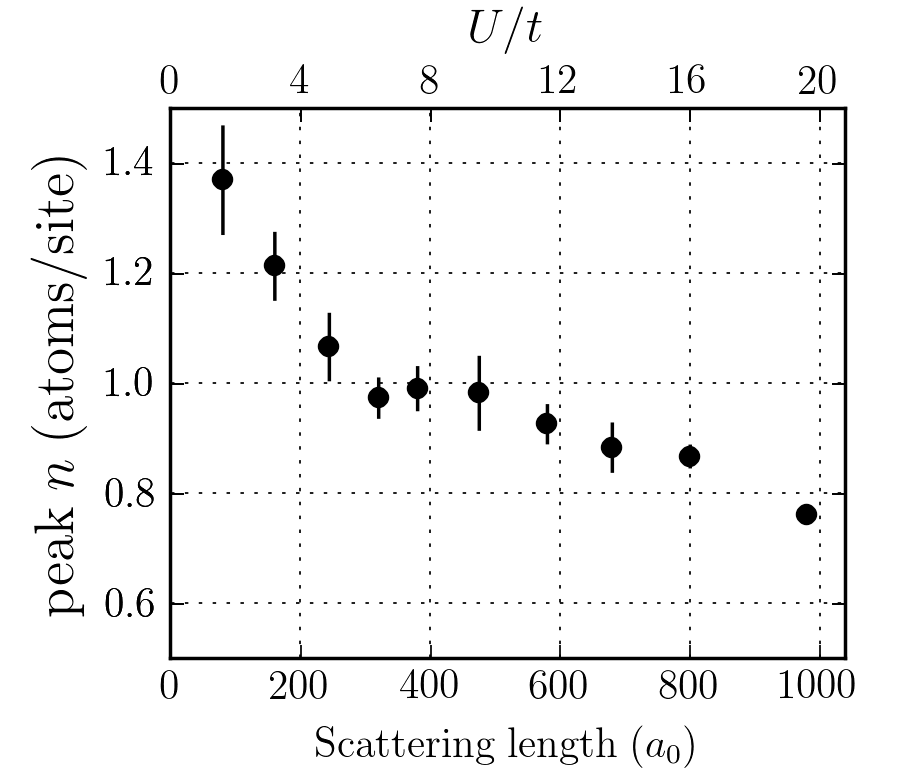
\includegraphics[width=0.5\textwidth]{../figures/double_occ/insitu_Dens.png}
\caption[Density measurement]{Measurement of the peak density of the cloud as a
function of scattering length in a compensated lattice. The preparation of the
sample is the same as for Fig.~8.3.  For scattering lengths between
300\,$a_{0}$ and 500\,$a_{0}$, the peak density is clamped at $n=1$ as the
interaction strength is increased.  This behavior is indicative of the system
entering the Mott insulating regime.  } 
\label{fig:dens-5.5Er}
\end{figure}

\section{\textit{In-situ} measurement of double occupancies}

Measurements taken at point $\boxed{4}$ address directly the double
occupancies.  In that case, \textit{in-situ} imaging would reveal the double
occupancy profile of the cloud.  It was not further investigated in this work,
but it is clear that important information can be extracted from the
\textit{in-situ} double occupancy profile, in the same way as can be extracted
from the \textit{in-situ} density profile (as showed in
Chapter~\ref{chap:mott}).  As an example we show a measurement in an
uncompensated lattice, with $N=75,000$ atoms in Fig.~\ref{fig:insitu-doublons}.  
\begin{figure}
\centering
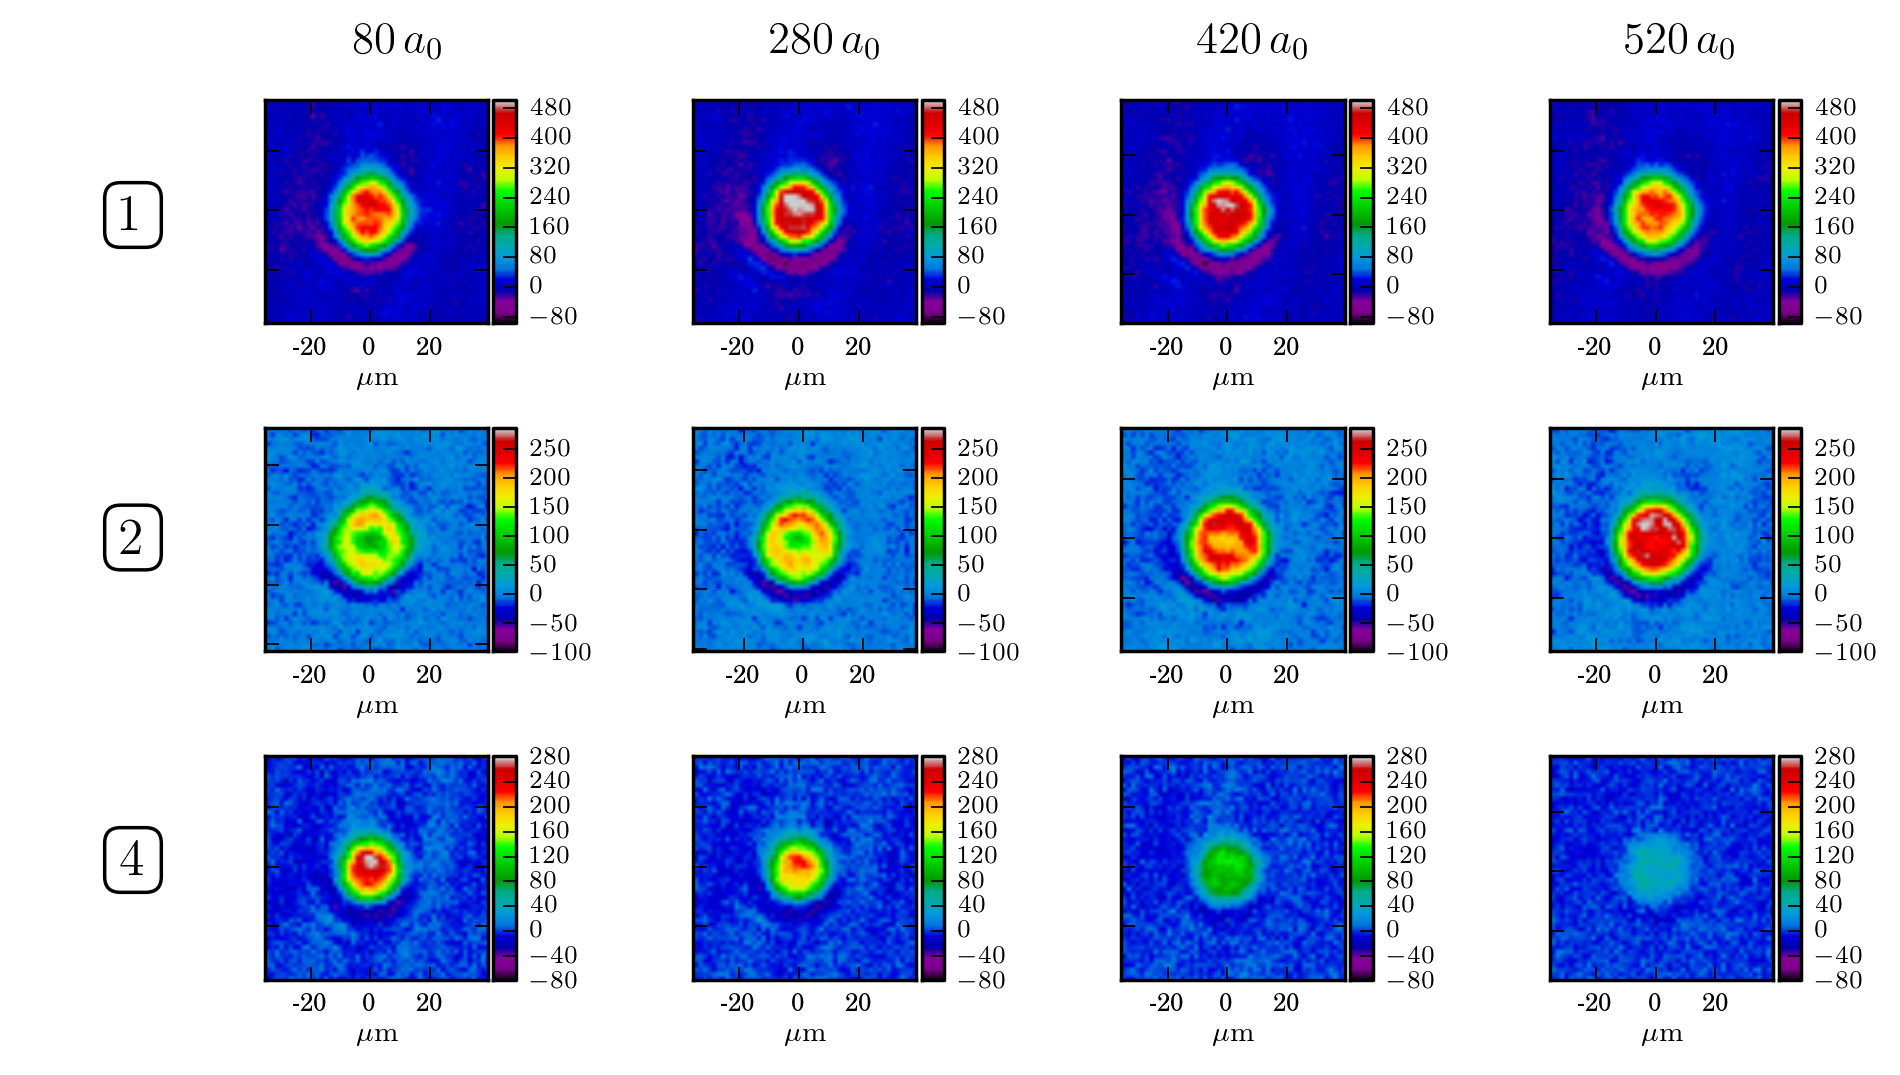
\includegraphics[width=\textwidth]{../figures/double_occ/doubleocc_Bstart100_k6_200_2Lock50_UncompLowNColumnDensity.png}
\caption[In-situ double occupancy measurement]{\textit{In-situ} measurement of
the double occupancy.  Images at points $\boxed{1}$, $\boxed{2}$, and
$\boxed{4}$ (as labeled in Fig.~\ref{fig:measure-doub}) are taken for various
scattering lengths.  One can see that the double occupancies are suppressed for
large scattering length, and that they reside at the center of the sample, as
expected.  We point out  that, even though we used a low number of atoms
($N=75,000$), a sample in the uncompensated lattice does not satisfy the
criteria for the single-band Hubbard model (due to the large confinement). At
the large resulting densities, significant dispersive distortions are
noticeable in the images (half-circle on the bottom part of the cloud). The
imaging detuning for these data is set at -120~MHz from state $|1\rangle$
(-44.5~MHz from state $|2\rangle$). } 
\label{fig:insitu-doublons}
\end{figure}

\section{Measurement systematics}

When measuring the double occupancies directly (point $\boxed{4}$ in
Fig.~\ref{fig:measure-doub})  one faces the issue that the molecules do not
have a long lifetime in the lattice.   Any amount of time that passes between
the molecular association and the image will result in a systematic error of
this measurement.   

In the descriptions above we also omitted an important fact.  We found that the
lifetime of the molecules is shortened dramatically in the presence of 532~nm
light (we use 532~nm for the compensation).   It is unclear what is the exact
decay mechanism for the molecules both in the presence or absence of 532~nm
light.   For measurements on a compensated lattice, like the one in
Fig.~\ref{fig:docc-5.5Er},  all of the 532~nm light was turned off after
locking the lattice and before starting the Feshbach association ramps to avoid
the extremely fast losses observed in the presence of 532~nm light.  

In the absence of 532~nm light, we measured the lifetime of the molecules by
varying the time between points $\boxed{2}$ and $\boxed{3}$ in the field ramps,
and observing the final number of dissociated atoms at point $\boxed{4}$.  The
details of the measurement are presented in Fig.~\ref{fig:molecule-lifetime}.
The observed lifetime was $\approx\,$100-200~ms, which is of the order of
magnitude of  the time it takes to make a direct measurement of the double
occupancy.    
\begin{figure}
\centering
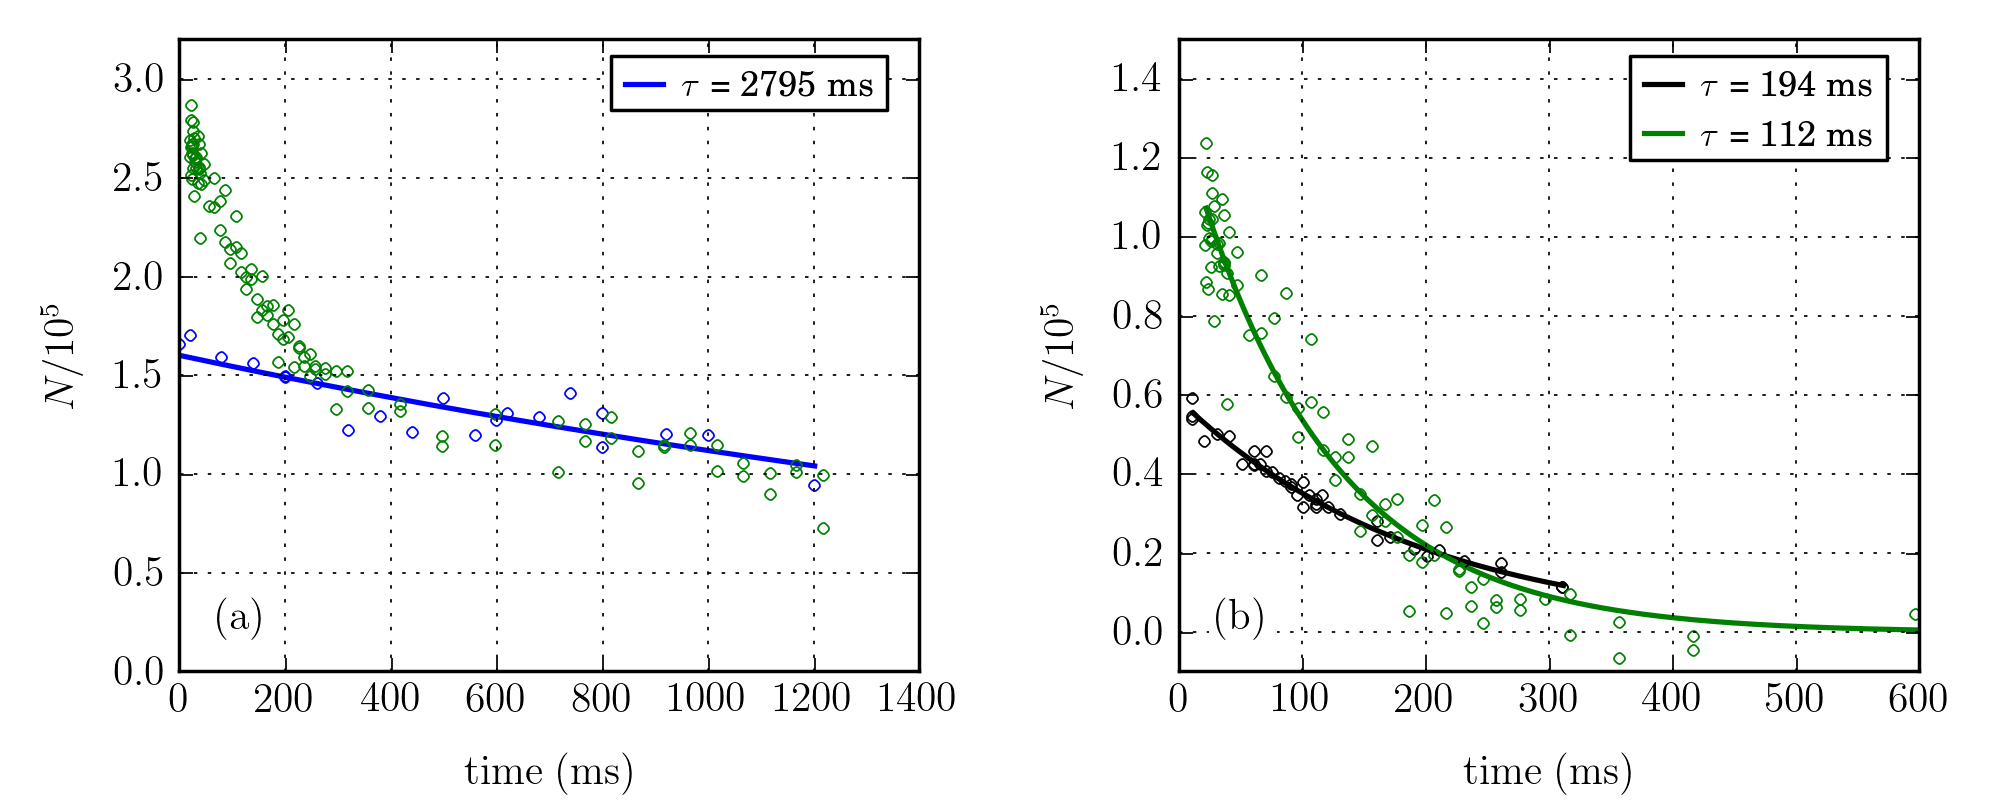
\includegraphics[width=\textwidth]{../figures/double_occ/lifetime_thesis.png}
\caption[Molecule lifetime]{Measurement of the lifetime of Feshbach molecules
in the uncompensated optical lattice.  The lattice was locked to 50\,$E_{r}$
for this measurement.  \vspace{0.5em}\newline  (a)  The blue points show a
reference loss curve taken at $a_{s}=48\,a_{0}$ after associating doubly
occupied sites into molecules (molecules here are dark to the imaging light).
The green points show a measurement taken at point $\boxed{4}$, after
dissociating molecules again such that they are not dark. The time is the hold
time between association and dissociation ramps, such that the molecular
lifetime can be extracted by comparing with the reference loss curve.  One can
see that the decay has a short time scale (lifetime of the molecules) and a
longer time scale which matches the blue points. \vspace{0.5em} \newline (b)
Green points are the same data in panel (a), with the long time scale decay
subtracted out.  Black points are a measurement taken at point $\boxed{4}$, in
which the atoms in singly occupied sites were blown away at point $\boxed{2}$.
In essence, the green shows the lifetime of molecules in the presence of singly
occupied sites and the black shows the lifetime of a sample made only of
molecules.  } 
\label{fig:molecule-lifetime}
\end{figure}

In addition to possible systematic due to molecule lifetime, we have found that
the sample gets affected when locking the lattice depth up to 50\,$E_{r}$.
Measurements of AFM correlations using Bragg scattering show that the
correlations effectively wash out for lock depths larger than $20\,E_{r}$.  It
is unclear why this happens;  in any case,  according to the results of AFM
correlations we cannot do a deep lattice lock without affecting the system.
This casts another shadow of doubt on the results of our double occupancy
measurements shown here, which use a lock depth of $50\,E_{r}$.   If we were to
reduce the lock depth to 20\,$E_{r}$, then the duration of the double occupancy
measurement would be comparable to the tunneling rate.    We speculate that in
a system with a large lattice beam waist, and with a beam waist ratio,
$\awaist$, closer to 1, the issues with the lock depth would be mitigated.  A
future setup, currently under construction, will help us get the answer to this
question. 





